
Każdy element graficznego interfejsu aplikacji (\emph{QWidget}) jest renderowany w momencie odebrania zdarzenia \emph{QPaintEvent} z kolejki zdarzeń głównego wątku aplikacji. Dzięki temu istnieje łatwy sposób na uzyskanie informacji o tym kiedy oraz ktory element należy przerenderować aby uaktualnić jego wygląd po stronie klienta. Problemem w dalszyb ciągu pozostaje jednak sposób na uzyskanie informacji o samym wyglądzie. 

\begin{figure}[H]
\centering
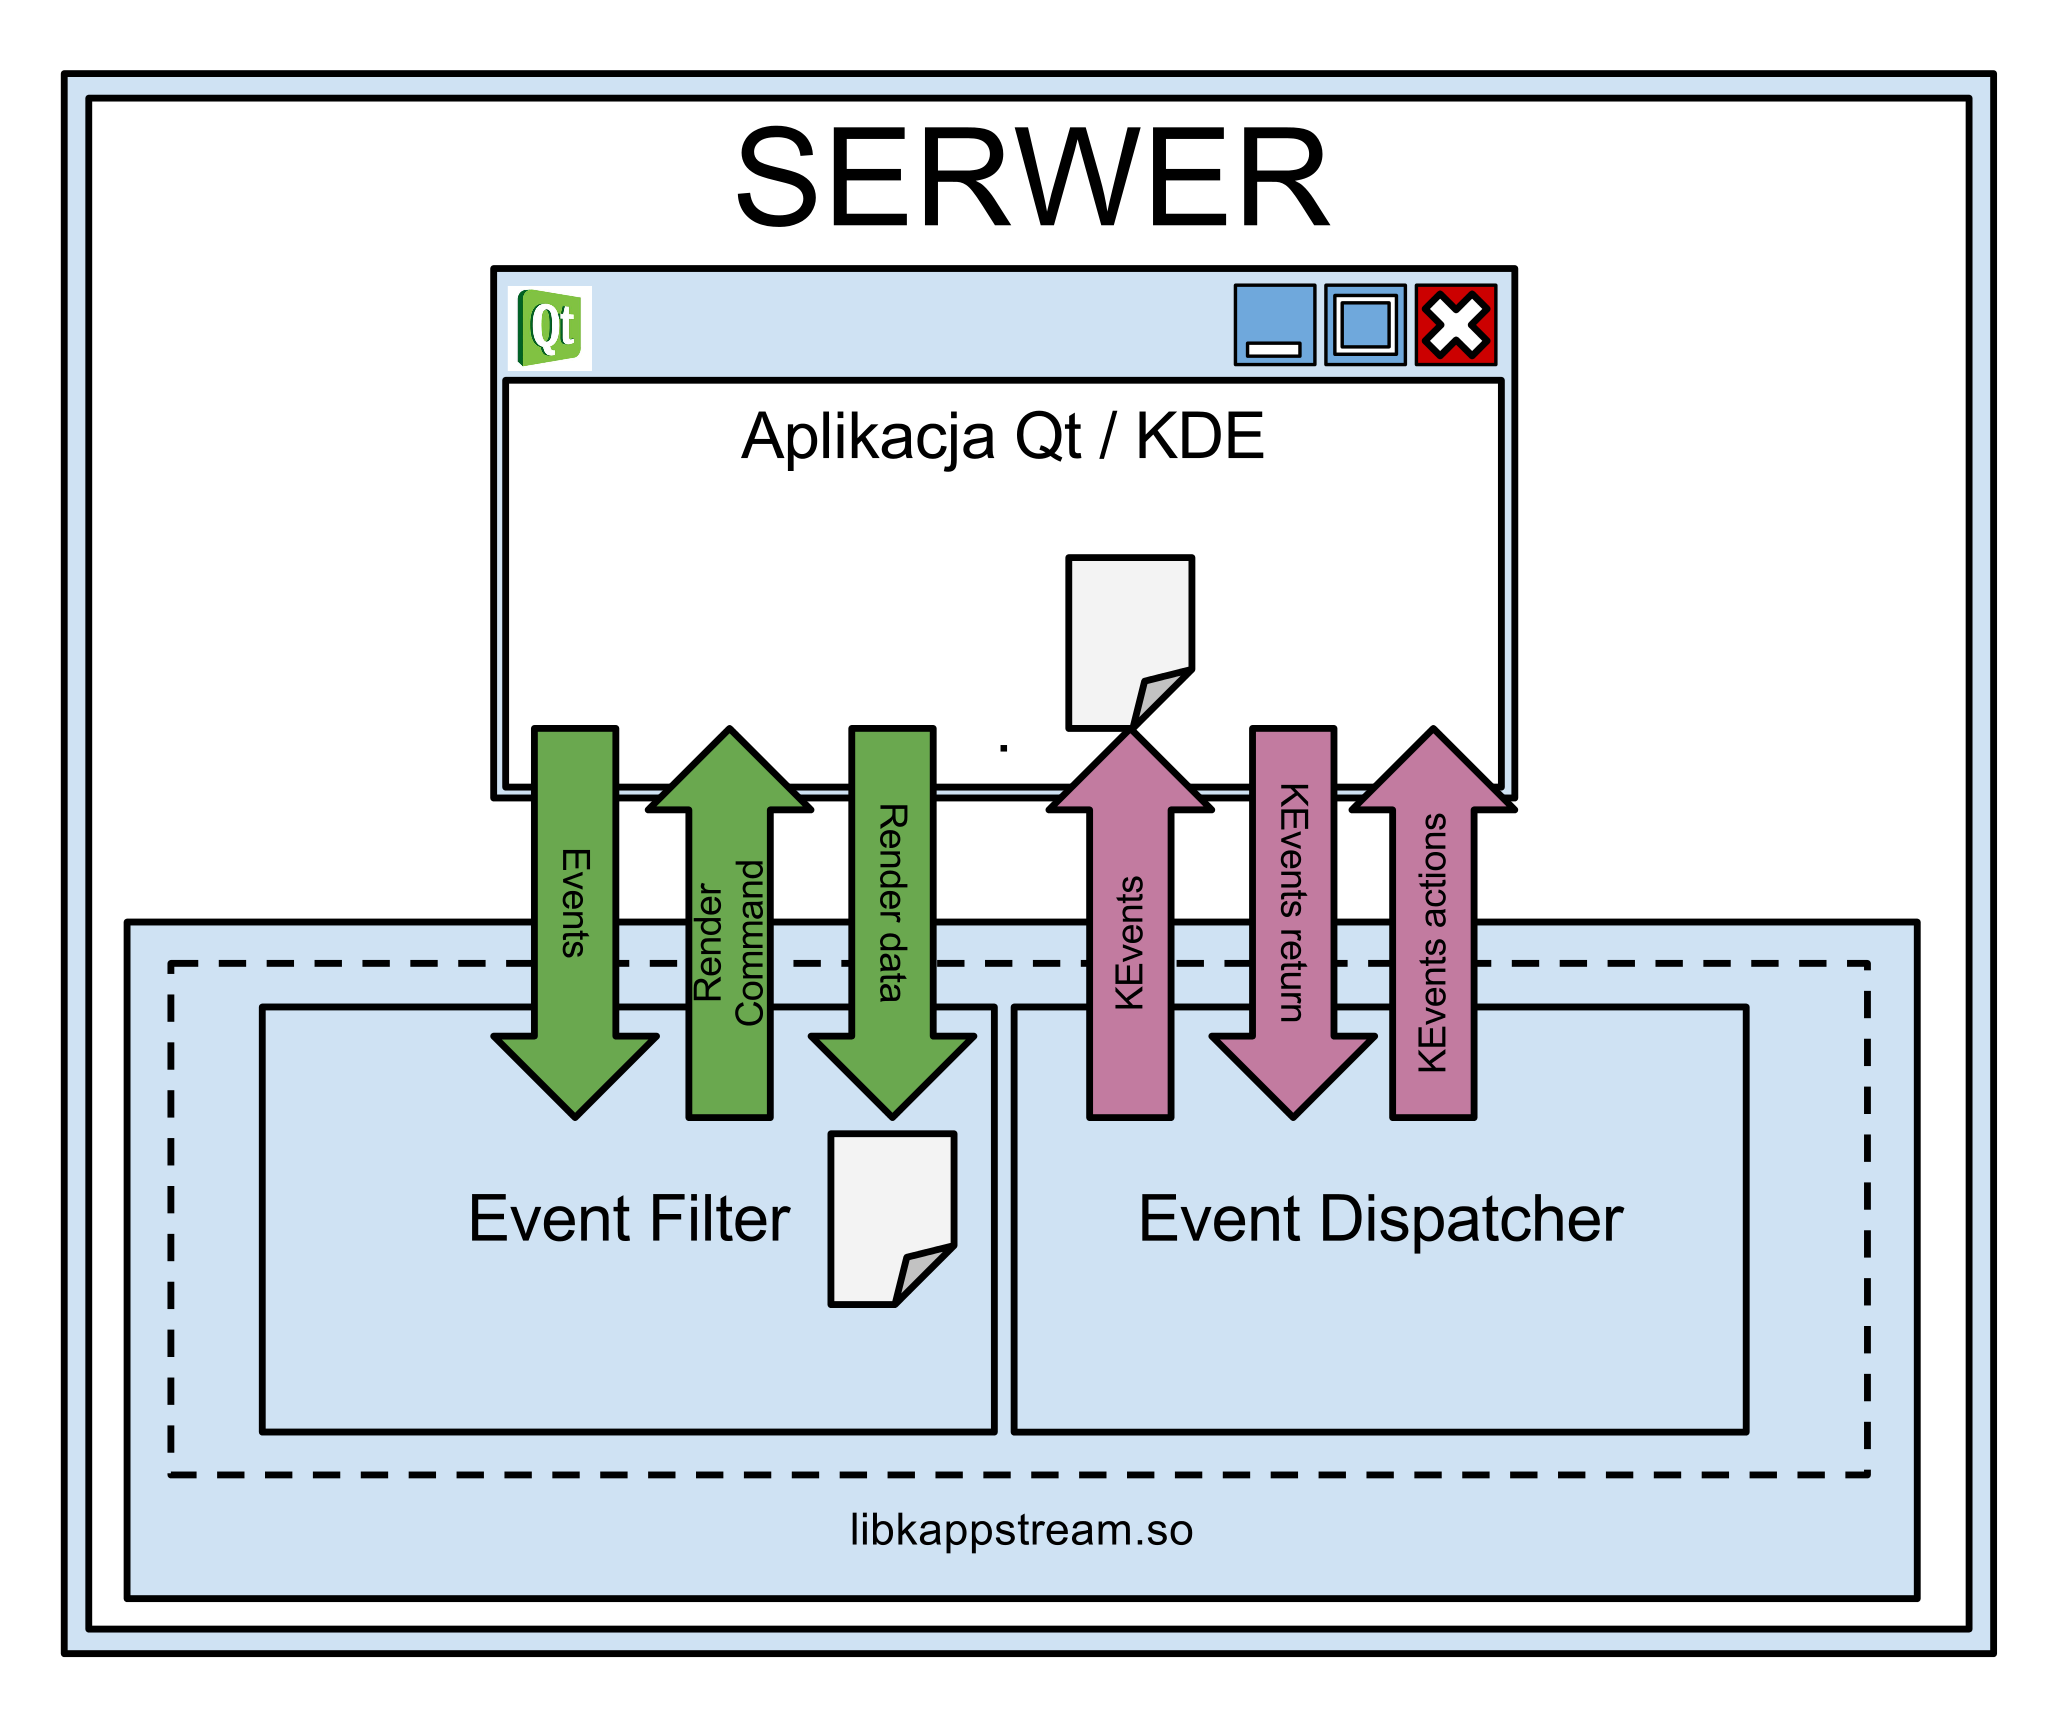
\includegraphics[width=1.0\linewidth]{img/arch-hook}
\caption{Schemat powiązań modułu WebSocket z aplikacją \emph{Qt/KDE}.}
\label{fig:arch-hook}
\end{figure}

Proponowane rozwiązanie polega na zaimplementowaniu abstrakcyjnego urządzenia wyjściowego reprezentującego przeglądarkę WWW po stronie klienta (patrz podrozdział \ref{system_rysowania}). Odpowiednio implementując klasy \emph{QPaintEngine} oraz \emph{QPaintDevice} możliwe staje się uzyskanie szczegółowych informacji dotyczących wygądu widgetów co z kolei umozliwia stworzenie innowacyjnego formatu przesyłanych danych. Jego innowacyjność polega na przerzuceniu odpowiedzialności za rysowanie elementów piksel po pikselu na stronę klienta na podstawie dostarczonych przez serwer niezbędnych do tego celu informacji. Zamiast przesyłać bitmapy z wyrenderowanym elementem można wysłać informacje o kolorach, punktach, liniach i innych podstawowych elementach, które zostaną narysowane na urządzeniu docelowym jakim po stronie klienta jest przeglądarka WWW z obsługą elementów \emph{canvas}. Na tle istniejących rozwiązań jest to podejście dotąd niespotykane.
